\documentclass{../beamercours}
\usepackage{tikz-3dplot}
\usepackage{pgfplots}
\usepackage{dsfont}


\title{Cours TalENS 2023-2024}
\subtitle{Dérivée, Volume, Aire, Périmètre}
\date{6 Avril 2024}

\begin{document}
\maketitle
\section{Rappels Mathématiques}
\subsection{Dérivation}
\begin{frame}{Dérivée par rapport à une variable}
\begin{définition}{Dérivabilité}{}
$f$ est dérivable si $f^{'}(x) = \lim\limits_{\mathrm{d}x \rightarrow 0} \frac{f(x + \mathrm{d}x) - f(x)}{\mathrm{d}x}$ existe. $f'(x)$ est la pente de la tangente à la courbe de $f$ en $x$.
\end{définition}
\visible<2->{
    \begin{propositionfr}{Règles de dérivation usuelles}{}
        \begin{itemize}[<+->]
            \item $\forall n \in \mathbb{Z},  \deriv{x}{x^{n}} = nx^{n-1}$
            \item $\deriv{x}{fg} = \deriv{x}{f}g + f\deriv{x}{g} $
        \end{itemize}
    \end{propositionfr}}
\end{frame}

\begin{frame}{Règle de la chaîne - Changement de Variable}
\begin{théorème}{Règle de la Chaîne}{}
Soit $f$ dérivable, $g$ dérivable : $\frac{\d}{\d x}(f(g(x))) = g'(x) \times f^{'}(g(x))$.
\end{théorème}
\begin{définition}{Changement de Variable}{}
On appelle poser dans $f$ le changement de $x = g(y)$ le fait d'écrire : $f(x) = f(g(y))$.\\ On a alors : $\deriv{x}{f(x)} = \deriv{x}{y}\deriv{x}{f(g(y))}$
\end{définition}

\end{frame}

\subsection{Polygones Réguliers et Solides de Platon}
\begin{frame}
\frametitle{Polygones Réguliers : Aire et Périmètre}
Un $n$-gone régulier est un polygone (convexe) à $n$ côtés de même longueur $c$.
\begin{théorème}{Formule de l'Aire et du Périmètre}{}
En notant $\rho$ l'apothème du polygone (la distance du centre à un côté) :
\begin{itemize}
    \item $P(n, c) = nc$
    \item $A(n, c) = n\frac{c\rho}{2} = P(n, c)\frac{\rho}{2}$
\end{itemize}
$\rho$ est une fonction de $c$.
\end{théorème}
\end{frame}

\begin{frame}
\frametitle{Un catalogue des Solides de Platon}
\begin{définition}{Solides de Platon}{}
Les solides de Platon sont les polyèdres réguliers convexes, i.e. des solides dont les faces sont planes polygonales régulières, similaires et se rencontrent selon des segemnts appelés arêtes.
\end{définition}
\visible<2>{
    \begin{center}
        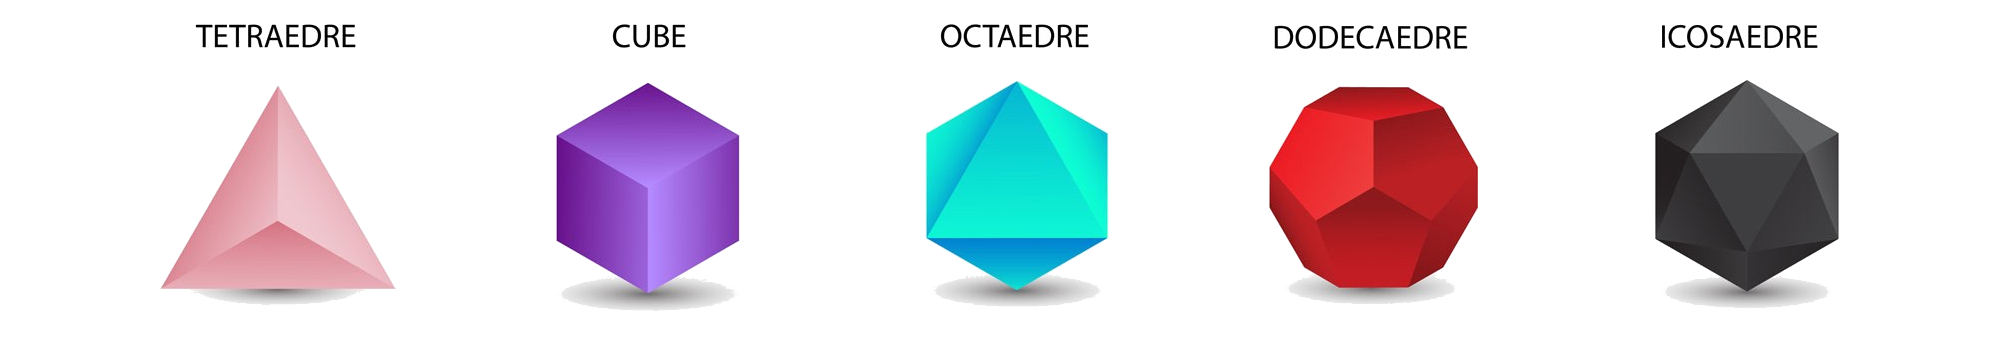
\includegraphics[width = \textwidth]{../Fichiers/solides-de-platon.png}
    \end{center}
}
\end{frame}

\begin{frame}
\frametitle{Exhaustivité}
\begin{théorème}{Liste des Solides de Platons}{}
Il y en a $5$ et seulement $5$: Le Tétraèdre (pyramide à 4 faces), le cube (hexaèdre), l'octaèdre, le dodécaèdre, l'icosaèdre.
\end{théorème}
\begin{proof}\small
    On a toujours : $S - A + F = 2$ et $pF = 2A = qS$, où $p$ est le nombre de côtés des faces, et $q$ le nombre de face se rejoignant à chaque sommet. 
    On en déduit qu'on doit avoir : $\frac{1}{p} + \frac{1}{q} > \frac{1}{2}$. Mais comme $p, q \geq 3$, on n'a bien que $5$ possibilités qui sont autant de solides.\\
\end{proof}
\end{frame}

\section{Constatations}
\subsection{En Dimension 2 et 3 : Le Cercle et la Sphère}
\begin{frame}
    \frametitle{Le Cercle}
    \begin{propositionfr}
        {Relation Rayon-Périmètre-Aire pour le Cercle}{}
        \begin{tabular}{m{.5\textwidth}m{4cm}}
            \begin{itemize}
                \item On a $P(\rho) = 2\pi\rho$
                \item On a $A(\rho) = \pi\rho^{2}$
                \item On a \[\frac{\d}{\d\rho}A(\rho) = P(\rho)\]
            \end{itemize} & 
            \centering
            \begin{tikzpicture}[scale = 1.1]
                \draw[->,] (-1.5cm,0cm) -- (1.5cm,0cm) node[right] {$x$};
                \draw[->] (0cm,-1.5cm) -- (0cm,1.5cm) node[above] {$y$};
                \draw[thick] (0cm,0cm) circle(1cm);
                \draw[->, thick, vulm!70!black] (0cm, 0cm) -- node[above] {$\rho$} (30:1cm);
            \end{tikzpicture}
        \end{tabular}
    \end{propositionfr}
\end{frame}


\tdplotsetmaincoords{60}{115}
\pgfplotsset{compat=newest}
\begin{frame}
    \frametitle{La Sphère}
    \begin{propositionfr}
        {Relation Rayon-Aire-Volume pour la Sphère}{}
        \begin{tabular}{m{.5\textwidth}m{4cm}}
            \begin{itemize}
                \item On a $A(\rho) = 4\pi\rho^{2}$
                \item On a $V(\rho) = \frac{4}{3}\pi\rho^{3}$
                \item On a \[\frac{\d}{\d\rho}V(\rho) = A(\rho)\]
            \end{itemize} & 
            \centering
            \begin{tikzpicture}[tdplot_main_coords, scale = 1.7]
                
                % Create a point (P)
                \coordinate (P) at ({1/sqrt(3)},{1/sqrt(3)},{1/sqrt(3)});
                
                % Draw shaded circle
                \shade[ball color = lightgray,
                    opacity = 0.5
                ] (0,0,0) circle (1cm);
                
                % draw arcs 
                \tdplotsetrotatedcoords{0}{0}{0};
                \draw[dashed,
                    tdplot_rotated_coords,
                    gray
                ] (0,0,0) circle (1);
                
                \tdplotsetrotatedcoords{90}{90}{90};
                \draw[dashed,
                    tdplot_rotated_coords,
                    gray
                ] (1,0,0) arc (0:180:1);
                
                \tdplotsetrotatedcoords{0}{90}{90};
                \draw[dashed,
                    tdplot_rotated_coords,
                    gray
                ] (1,0,0) arc (0:180:1);
                
                % % Projection of the point on X and y axes
                % \draw[thin, dashed] (P) --++ (0,0,{-1/sqrt(3)});
                % \draw[thin, dashed] ({1/sqrt(3)},{1/sqrt(3)},0) --++
                % (0,{-1/sqrt(3)},0);
                % \draw[thin, dashed] ({1/sqrt(3)},{1/sqrt(3)},0) --++
                % ({-1/sqrt(3)},0,0);
                
                % Axes in 3 d coordinate system
                \draw[-stealth] (0,0,0) -- (1.80,0,0);
                \draw[-stealth] (0,0,0) -- (0,1.30,0);
                \draw[-stealth] (0,0,0) -- (0,0,1.30);
                \draw[dashed, gray] (0,0,0) -- (-1,0,0);
                \draw[dashed, gray] (0,0,0) -- (0,-1,0);
                
                % Line from the origin to (P)
                \draw[thick, -stealth, vulm!70!black] (0,0,0) --node[above]{$\rho$} (P);
                
            \end{tikzpicture}
        \end{tabular}
    \end{propositionfr}
\end{frame}

\subsection{Presque Contre-Exemples}
\begin{frame}
    \frametitle{Le Carré}
    \begin{propositionfr}
        {Relation Rayon-Périmètre-Aire pour le Carré}{}
        \begin{tabular}{m{.5\textwidth}m{4cm}}
            \begin{itemize}
                \item On a $P(\rho) = 4c$
                \item On a $A(\rho) = c^{2}$
                \item On a \[\frac{\d}{\d\rho}A(\rho) = \frac{1}{2}P(\rho)\]
            \end{itemize} & 
            \centering
            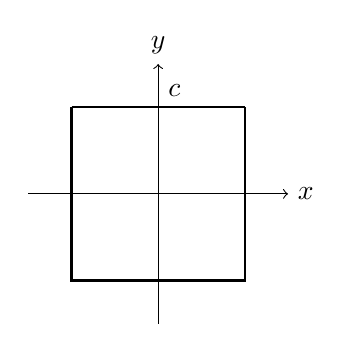
\begin{tikzpicture}[scale = 1.1]
                \draw[->,] (-1.5cm,0cm) -- (1.5cm,0cm) node[right] {$x$};
                \draw[->] (0cm,-1.5cm) -- (0cm,1.5cm) node[above] {$y$};
                \draw[thick] (-1cm, 1cm) -- node[above right] {$c$} (1cm, 1cm);
                \draw[thick] (1cm, 1cm) -- (1cm, -1cm) -- (-1cm, -1cm) -- (-1cm, 1cm);
            \end{tikzpicture}
        \end{tabular}
    \end{propositionfr}
\end{frame}

\begin{frame}
    \frametitle{Le Triangle Equilatéral}
    \begin{propositionfr}
        {Relation Rayon-Périmètre-Aire pour le Triangle}{}
        \begin{tabular}{m{.5\textwidth}m{4cm}}
            \begin{itemize}
                \item On a $P(\rho) = 3c$
                \item On a $A(\rho) = \frac{\sqrt{3}}{4}c^{2}$
                \item On a \[\frac{\d}{\d\rho}A(\rho) = \frac{2}{\sqrt{3}}P(\rho)\]
            \end{itemize} & 
            \centering
            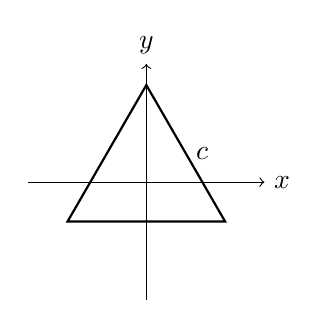
\begin{tikzpicture}[scale = 1]
                \draw[->,] (-1.5cm,0cm) -- (1.5cm,0cm) node[right] {$x$};
                \draw[->] (0cm,-1.5cm) -- (0cm,1.5cm) node[above] {$y$};
                \draw[thick] (-1cm, -.5cm) -- (0, 1.232) -- node[right] {$c$} (1cm, -.5cm) -- cycle;
            \end{tikzpicture}
        \end{tabular}
    \end{propositionfr}
\end{frame}

\begin{frame}
    \frametitle{Le Cube}
    \begin{propositionfr}
        {Relation Rayon-Périmètre-Aire pour le Khûbe}{}
        \begin{tabular}{m{.5\textwidth}m{4cm}}
            \begin{itemize}
                \item On a $A(\rho) = 6c^{2}$
                \item On a $V(\rho) = c^{3}$
                \item On a \[\frac{\d}{\d\rho}V(\rho) = \frac{1}{2}A(\rho)\]
            \end{itemize} & 
            \centering
            \tdplotsetmaincoords{60}{125}
            \begin{tikzpicture}
                [tdplot_main_coords, scale = .8,
                    cube/.style={thick,black},
                    grid/.style={very thin,gray},
                    axis/.style={->}]
                
                %draw a grid in the x-y plane
                \foreach \x in {-0.5,0,...,2.5}
                \foreach \y in {-0.5,0,...,2.5}
                    {
                        \draw[grid] (\x,-0.5) -- (\x,2.5);
                        \draw[grid] (-0.5,\y) -- (2.5,\y);
                    }
                
                
                %draw the axes
                \draw[axis] (0,0,0) -- (3,0,0) node[anchor=north]{$x$};
                \draw[axis] (0,0,0) -- (0,3,0) node[anchor=north]{$y$};
                \draw[axis] (0,0,0) -- (0,0,3) node[anchor=west]{$z$};
                
                %draw the top and bottom of the cube
                \draw[cube] (0,0,0) -- (0,2,0) -- (2,2,0) -- (2,0,0) -- cycle;
                \draw[cube] (0,0,2) -- node[above]{$c$} (0,2,2) -- (2,2,2) -- (2,0,2) -- cycle;
                
                %draw the edges of the cube
                \draw[cube] (0,0,0) -- (0,0,2);
                \draw[cube] (0,2,0) -- (0,2,2);
                \draw[cube] (2,0,0) -- (2,0,2);
                \draw[cube] (2,2,0) -- (2,2,2);
                
            \end{tikzpicture}
        \end{tabular}
    \end{propositionfr}
\end{frame}

\section{Généralisation}

\subsection{L'Aire et le Volume en Plus que 3 Dimensions}
\begin{frame}{Un Solide en $d$ Dimensions}
    \begin{définition}
        {Solide à $d$ Dimensions}{}
        On appelle Solide à $d$ Dimensions une partie compacte dont les bords sont de mesure finie de l'espace à $d$ dimensions.
    \end{définition}    
    \visible<2->{
        On rappelle que la mesure d'un ensemble est sa \textit{taille} par rapport à l'espace dans lequel il vit.
    }
\end{frame}

\begin{frame}{Mesure de Lebesgue et Volume}
    \begin{définition}
        {Volume d'un Pavé}{}
        Pour $\mathcal{P} = [a_{1}, b_{1}] \times \cdots \times [a_{d}, b_{d}]$ un pavé, on définit son volume:
        \[
            V(\mathcal{P}) = \prod_{i = 1}^{n} \abs{b_{i} - a_{i}}
        \]
    \end{définition}
    \visible<2>{
        \begin{théorème}
            {Mesure de Lebesgue}{}
            Il existe une unique mesure sur $\R^{d}$ qui soit complète et coïncide sur les pavés avec leur volume. On la note $\lambda_{d}$.
        \end{théorème}
    }
\end{frame}
\begin{frame}
    \frametitle{Aire et Volume en $d$ Dimensions}
    \begin{définition}
        {Volume et Aire d'une Partie}{}
        Étant donnée une partie $\mathcal{P}$ de $\R^{d}$, on définit son volume par 
        \begin{equation*}
            V(\mathcal{P}) = \lambda_{d}(\mathcal{P}) =  \int_{\R^{d}} \mathds{1}_{\mathcal{P}}\d\lambda_{d}
        \end{equation*}
        On définit de même son aire $A(\mathcal{P})$ par 
        \begin{equation*}
            A(\mathcal{P}) = \lambda_{d - 1}(\partial\mathcal{P})
        \end{equation*}
    \end{définition}
\end{frame}

\subsection{Formalisation}
\begin{frame}
    \frametitle{Famille de Lisse de Formes Uni-Paramétrées}
    On considère $\mathcal{F}$ une famille de formes uni-paramétrées sur un intervalle $E$ de $\R$: 
    \begin{equation*}
        \mathcal{F} = \left\{R(s) \subset \R^{d}\ \middle|\ s \in E\right\}
    \end{equation*}
    On suppose que cette famille vient avec une fonction dérivable strictement croissante de volume $V: E \to \R^{+}$ et une fonction continue d'aire $A: E \to \R^{+}$.\\
    \visible<2>{
        Par exemple, pour les carrés de côté $> 0$, $\mathcal{C} =\left\{[0, c] \times [0, c] \subset \R^{2}\ \middle|\ s \in [0, +\infty[\right\}$, $V : s\mapsto s^{2}$ et $A : s \mapsto 6s$.
    }
\end{frame}

\begin{frame}
    \frametitle{Dérivée du Volume par Rapport à...}
    \begin{théorème}
        {Relation de Dérivation Volume-Aire}{}
        Soit $\mathcal{F}$ une famille uni-paramétrée lisse de régions compactes de l'espace. Alors, il y a un changement de variable dérivable $r(s) : E \to r(E)$ défini par
        \vspace{-3pt}
        \begin{equation*}
            r(s) = \int \frac{V'(s)}{A(s)}\d s
        \end{equation*}
        \vspace{-4pt}
        unique à constante près tel que 
        \vspace{-4pt}
        \begin{equation*}
            \frac{\d}{\d r}V[s(r)] = A[s(r)], r \in r(E)
        \end{equation*}
    \end{théorème}
\end{frame}

\begin{frame}
    \frametitle{Preuve du Théorème Précédent}
    \begin{proof}
        Puisque $V$ est monotone et $A$ est positive, le signe de \vspace{-5pt}
        \begin{equation*}
            r'(s) = \frac{V'(s)}{A(s)}\vspace{-5pt}
        \end{equation*}
        est constant et $r$ est un changement de variable dérivable de $E$ dans $r(E)$.\\
        Par la règle de la chaîne: 
        \vspace{-5pt}
        \begin{equation*}
            \frac{\d}{\d r}V[s(r)] = V'[s(r)]s'(r) = \frac{V'[s(r)]}{r'[s(r)]} = A[s(r)]\vspace{-5pt}
        \end{equation*}
    \end{proof}
\end{frame}

\begin{frame}
    \frametitle{Interprétation Géométrique - 1}
    \begin{itemize}[<+->]
        \item Pour une famille de carrés, $r(s) = \frac{s}{2} + k,  k \in \R^{+}$
        \item Pour une famille de cubes, $r(s) = \frac{s}{2} + k$
        \item Pour une famille de rectangles de largeur $a > 0$ et de longueur $s$, \[r(s) = \frac{a}{s}\ln(2s + 2a) + k\]
        \item Pour une famille de rectangles de longueur $s$ et de largeur $as$ où $0 < a < 1$, \[r(s) = \frac{a}{a + 1}s + k\]
    \end{itemize}
\end{frame}

\begin{frame}
    \frametitle{Interprétation Géométrique - 2}
    \begin{théorème}
        {Famille Homogène}{}
        Dans le cas où $V$ et $A$ sont homogènes de degré $d$ et $d - 1$, i.e. $V(ts) = t^{d}V(s)$ et $A(ts) = t^{d-1}A(s)$, on a $r(s) = \d \frac{V(s)}{A(s)}$.
    \end{théorème}

    \begin{théorème}
        {Interprétation Géométrique}{}
        Si $P$ est un polytope de volume $V$ et d'aire $A$ qu'on dilate d'une distance $r$ centrée en $p$. On a alors \vspace{-5pt}
        \begin{equation*}
            \frac{\d V}{\d r} = A \Longleftrightarrow \mathbb{S}(p, r) \subseteq P\vspace{-3pt}
        \end{equation*}
    \end{théorème}
\end{frame}

\begin{frame}
	\frametitle{Preuve}
	\begin{proof}
		\only<1>{
		Soit $V$ le volume d'un polytope $P$ dont les faces sont d'aires $A_{i}$. 
		On considère des cônes du point arbitraire $p$ de $P$ vers les faces de $O$ et on prend $r$ un rayon provisoire à la face la plus proche, d'aire $A_{0}$.\\
		Il existe des constantes $a_{i}$ et $k_{i}$ telles que $A_{i} = a_{i}A_{0}$ et $h_{i} = k_{i}r$ où $h_{i}$ est la hauteur du $i$-ème cône. 
		Ces relations subsistent par dilatation et on a toujours $k_{i} \geq 1$.}
		\only<2>{
		Notons que $A = \sum_{i} A_{i} = \left(\sum_{i}a_{i}\right)A_{0}$. De plus:\vspace{-6pt} 
		\begin{equation*}
			\begin{aligned}
				\frac{\d V}{\d r} =& \sum \frac{\d V_{i}}{\d r} = \sum \frac{\d V_{i}}{\d h_{i}} = \sum k_{i}A_{i}\\
				=& \sum k_{i}a_{i} A_{0} = \frac{\sum a_{i}k_{i}}{\sum a_{i}}\left(\sum a_{i}\right)A_{0}\\
				=& \frac{\sum k_{i}a_{i}}{\sum a_{i}}A\vspace{-10pt}
			\end{aligned}
		\end{equation*}
		On choisit alors un point qui minimise ce facteur en une valeur supérieure ou égale à $1$. Celle-ci vaut $1$ si tous les $k_{i}$ valent $1$, c'est à dire si $P$ circonscrit la sphère de centre $p$ et de rayon $r$. 
	}
	\end{proof}
\end{frame}


\begin{frame}
    \frametitle{Bibliographie}
    \nocite{*}
    \bibliography{Cours_Dérivée_Aire}
    \bibliographystyle{alpha}
\end{frame}

\end{document}
